\documentclass[journal]{IEEEtran}
\usepackage[a5paper, margin=10mm]{geometry}
%\usepackage{lmodern} % Ensure lmodern is loaded for pdflatex
\usepackage{tfrupee} % Include tfrupee package

%iffalse
\let\negmedspace\undefined
\let\negthickspace\undefined
\usepackage{gvv-book}
\usepackage{gvv}
\usepackage{cite}
\usepackage{amsmath,amssymb,amsfonts,amsthm}
\usepackage{algorithmic}
\usepackage{graphicx}
\usepackage{textcomp}
\usepackage{xcolor}
\usepackage{txfonts}
\usepackage{listings}
\usepackage{enumitem}
\usepackage{mathtools}
\usepackage{gensymb}
\usepackage{comment}
\usepackage[breaklinks=true]{hyperref}
\usepackage{tkz-euclide} 
\usepackage{listings}                                        
%\def\inputGnumericTable{}                                 
\usepackage[latin1]{inputenc}                                
\usepackage{color}                                            
\usepackage{array}                                            
\usepackage{longtable}                                       
\usepackage{calc}                                             
\usepackage{multirow}                                         
\usepackage{hhline}                                           
\usepackage{ifthen}                                           
\usepackage{lscape}
\usepackage{tabularx}
\usepackage{array}
\usepackage{float}
\usepackage{multicol}

\newcommand{\BEQA}{\begin{eqnarray}}
\newcommand{\EEQA}{\end{eqnarray}}
%\newcommand{\define}{\stackrel{\triangle}{=}}

\setlength{\headheight}{1cm} % Set the height of the header box
\setlength{\headsep}{0mm}     % Set the distance between the header box and the top of the text

%\usepackage[a5paper, top=10mm, bottom=10mm, left=10mm, right=10mm]{geometry}


\setlength{\intextsep}{10pt} % Space between text and floats

% Marks the beginning of the document
\begin{document}
\onecolumn
\bibliographystyle{IEEEtran}
\vspace{3cm}

%\renewcommand{\theequation}{\theenumi}
\numberwithin{equation}{section}
\numberwithin{figure}{section}
% \renewcommand{\thefigure}{\theenumi}
\renewcommand{\thetable}{\theenumi}

\title{A logo for Narayanpal}
\author{Subhodeep Chakraborty, Shiven Bajpai and G.V.V. Sharma}
\maketitle

% \renewcommand{\thefigure}{\theenumi}
\renewcommand{\thetable}{\theenumi} 

\setcounter{section}{1}
\textbf{Question: } Given that
\begin{align}
	f(t) &= e^{-at}u(t) + e^{bt}u(-t) \label{q1}\\
	u(t) &= \begin{cases}
		0, & t<0\\
		\frac{1}{2}, & t=0 \\
		1, & t>0
	\end{cases} \label{q2}\\
	\int_{-\infty}^{\infty} f(t) &= 1 \label{q3}
\end{align}

Find the possible values of $(a,b)$ if these are the end points of the latus recta of the associated conic. Plot $f(t)$ for these values of $(a,b)$

\bigskip

\textbf{Solution: } We expand the integral as 

\begin{align}
	\int_{-\infty}^{\infty} f(t) &= \int_{-\infty}^{0} f(t) + \int_{0}^{\infty} f(t)\\
	&= \int_{-\infty}^{0} e^{bt} + \int_{0}^{\infty} e^{-at}\\
	&= \frac{1}{b} + \frac{1}{a} \label{integral_result}
\end{align}

Subsituting \eqref{q3} in \eqref{integral_result}

\begin{align}
	\frac{1}{a} + \frac{1}{b} &= 1 \label{eq:cond_ab}\\
	ab - a - b &= 0 \label{conic_ab}
\end{align}

Which is the equation of a conic. 
If we take $a$ to be $x$ and $b$ to be $y$ and then express this as a conic in standard form \eqref{eq:app-conic_quad_form} we get

\begin{align}
	\text{g}(\vec{x}) = \vec{x}^\text{T}\vec{Vx} + 2\vec{u}^\text{T}\vec{x} + f \label{actual_conic}
\end{align}

By comparison we obtain:

\begin{align}
	\vec{V} &= \myvec{0 & \frac{1}{2} \\ \frac{1}{2} & 0}\\
	\vec{u} &= \myvec{-\frac{1}{2} \\ -\frac{1}{2}}\\
	f &= 0
\end{align}

We eigen decompose $\vec{V}$ \eqref{eq:conic_eig_def} as 

\begin{align}
	\vec{V} &= \vec{PDP}^\text{T}\\
	\vec{P} &= \myvec{\frac{1}{\sqrt{2}} & \frac{-1}{\sqrt{2}} \\ \frac{1}{\sqrt{2}} & \frac{1}{\sqrt{2}}}\\
	\vec{D} &= \myvec{\frac{1}{2} & 0 \\ 0 & \frac{-1}{2}}
\end{align}

And convert the conic into a standard conic \eqref{eq:app-conic_simp_temp_nonparab} to make it simpler to solve using affine transformations~\eqref{eq:conic_affine}.

\begin{align}
	\vec{y}^\text{T}\brak{\frac{\vec{D}}{f_0}}\vec{y} &= 1\\
	\vec{x} &= \vec{Py} + \vec{c} \label{t1}\\
\end{align}

Where 

\begin{align}
	f_0 &= \vec{u}^\text{T}\vec{V}^{-1}\vec{u} - f = 1\\
	\vec{c} &= -\vec{V}^{-1}\vec{u} = \myvec{1 \\ 1}
\end{align}

Since eigenvalues of $\vec{D}$ are $\lambda_1 = \frac{1}{2}$ and $\lambda_2=-\frac{1}{2}$ We use another transformation to shift the negative eigenvalue of $\vec{D}$ to get the hyperbola in standard form, finally giving us

\begin{align}
	\vec{z}^\text{T}\brak{\frac{\vec{D_0}}{f_0}}\vec{z} &= 1\\
	j(\vec{z}) = \vec{z}^\text{T}\vec{D_0}\vec{z} - f_0 &= 0  \label{standard_conic}\\
	\vec{y} &= \vec{P}_0\vec{z} \label{t2}\\
\end{align}

Here $\vec{P}_0$ is the reflection matrix $\myvec{0 & 1 \\ 1 & 0}$ and $\vec{D}_0$ is defined as 

\begin{align}
	\vec{D} &= \vec{P}_0\vec{D}_0\vec{P}_0^\text{T}\\
	\vec{P}_0^\text{T}\vec{D}\vec{P}_0 &= \vec{D}_0\\
	\vec{D}_0 &= \myvec{\frac{-1}{2} & 0 \\ 0 & \frac{1}{2}}
\end{align}

Now we solve to find the endpoints of the latus recta of this standard conic (\appref{app:conic-parameters})

\begin{align}
	\vec{n} &= \sqrt{\lambda_2}\vec{p}_1 = \myvec{0 \\ \frac{1}{\sqrt{2}}}\\
	e &= \sqrt{1 - \frac{\lambda_1}{\lambda_2}} = \sqrt{2}\\
	c &= \dfrac{e\vec{u}^\text{T}\vec{n} \pm \sqrt{e^2 (\vec{u}^T \vec{n})^2 - \lambda_2(e^2 - 1)(\Vert \vec{u} \Vert^2-\lambda_2f)}}{\lambda_2e(e^2 - 1)}\\
	&= \pm \frac{1}{\sqrt{2}}\\
	\vec{F} &= \dfrac{ce^2\vec{n}-\vec{u}}{\lambda_2} = \pm 2 \vec{e}_2\\
\end{align}

Equation of latus recta is

\begin{align}
	\vec{n}^\text{T}\vec{x} &= \vec{n}^\text{T}\vec{F}\\
	\equiv \vec{n}^\text{T}\vec{x} &= \sqrt{2}\\
	\equiv \vec{x} &= \vec{h} + k\vec{m} \label{latus_rectum}\\
	\vec{h} &= \myvec{0 \\ \pm 2}\\
	\vec{m} &= \myvec{1 \\ 0}
\end{align}

Let $\vec{\hat{z}}$ be the endpoints of the latus recta i.e the intersection of \eqref{latus_rectum} with the conic \eqref{standard_conic}, solved in \ref{prop:chord}

\begin{align}
	k &= \frac{1}{\vec{m}^\text{T}\vec{D_0}\vec{m}} \brak{-\vec{m}^\text{T}(\vec{D_0h} + \vec{u_0}) \pm \sqrt{\sbrak{\vec{m}^\text{T}(\vec{D_0h} + \vec{u_0})}^2 - j(\vec{h}) (\vec{m}^\text{T}\vec{D_0m})}}\\
	&= \pm \sqrt{2}\\
	\therefore \vec{\hat{z}} &= \myvec{\pm \sqrt{2} \\ \pm 2}
\end{align}

% From \eqref{latus_rectum} we can say $\vec{\hat{z}}$ is of the form $\myvec{k_i \\ \pm2}$. Subsituting back in \eqref{standard_conic}

% \begin{align}
% 	\vec{z}^\text{T}\vec{D_0}\vec{z} - f_0 &= 0\\
% 	-\frac{k_i^2}{2} + 2 - 1 &= 0\\
% 	k_i^2 &= 2\\
% 	k_i &= \pm \sqrt{2}\\
% 	\therefore \vec{\hat{z}} &= \myvec{\pm \sqrt{2} \\ \pm 2}
% \end{align}

Now transforming $\vec{\hat{z}}$ back using \eqref{t1}, \eqref{t2} to get endpoints of original conic $\vec{\hat{x}}$.

\begin{align}
	\vec{\hat{x}} &= \vec{P}\brak{\vec{P}_0 \vec{\hat{z}}} + \vec{c}
\end{align}

Which gives us values of $\vec{\hat{x}}$ to be

\begin{align*}
	\vec{\hat{x}}_1 &= \myvec{2+\sqrt{2} \\ \sqrt{2}}\\
	\vec{\hat{x}}_2 &= \myvec{\sqrt{2} \\ 2+\sqrt{2}}\\
	\vec{\hat{x}}_3 &= \myvec{2-\sqrt{2} \\ -\sqrt{2}}\\
	\vec{\hat{x}}_4 &= \myvec{-\sqrt{2} \\ 2-\sqrt{2}}
\end{align*}

We can plot out the original conic in \eqref{actual_conic} to verify our solution

\begin{figure}[H]
	\centering
	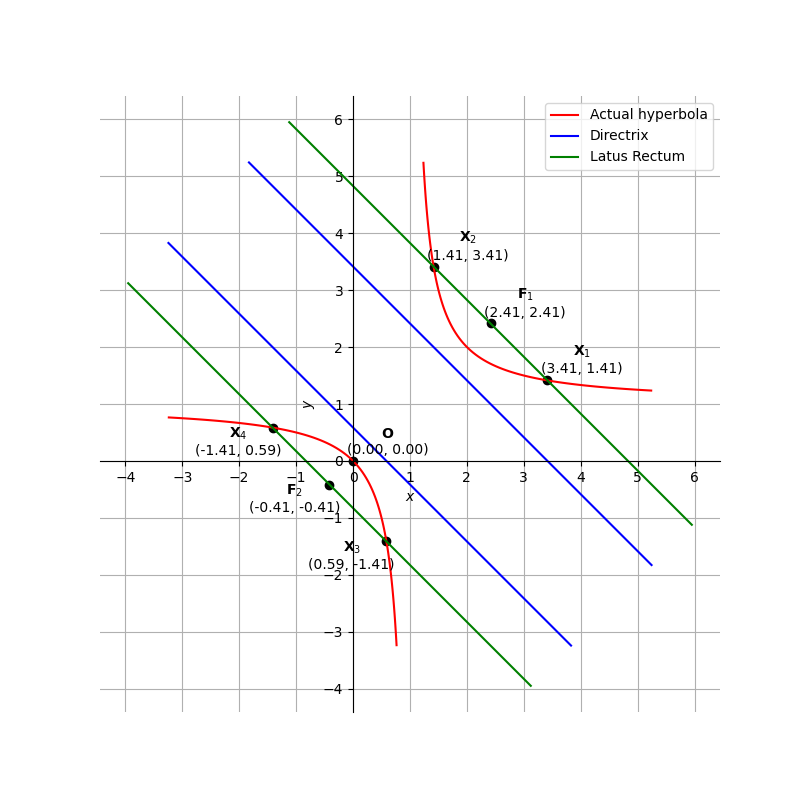
\includegraphics[width=0.75\columnwidth]{figs/Hyperbola.png} 
	\caption{}
	\label{fig:Hyperbola}
\end{figure}

Out of these, $\vec{\hat{x}}_3$ and $\vec{\hat{x}}_4$ are unfit to be used as values for $(a, b)$ as negative values of $a$ or $b$ will cause $f(t)$ to not be finite and thus the integral in \eqref{q3} will not converge and condition will not be met.\\

Lastly, We plot the function $f(t)$ for $(a, b) = \vec{\hat{x}}_1$ and $(a, b) = \vec{\hat{x}}_2$

\begin{figure}[H]
	\centering
	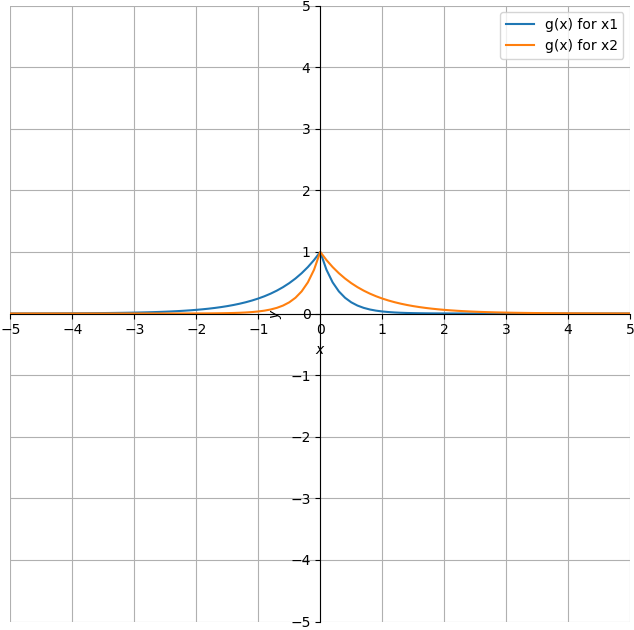
\includegraphics[width=0.75\columnwidth]{figs/function.png} 
	\caption{}
	\label{fig:Function}
\end{figure} 

\iffalse
Code for Figures \ref{fig:Hyperbola} and \ref{fig:Function} can be found at:
\begin{lstlisting}
Codes/solution.py
\end{lstlisting}
\fi
\section{Derivation of Truncation Points}
To plot the function $f(t)$ effectively, we define truncation points $t_1$ and $t_2$ such that a fraction $p$ of the total area is retained. Given $f(t)$ from \eqref{q1} and \eqref{q2}:
\begin{align}
    f(t) = \begin{cases} 
        e^{bt}, & t < 0 \\
        e^{-at}, & t > 0 
    \end{cases}
\end{align}
The total area is $A = \int_{-\infty}^{\infty} f(t)dt = \frac{1}{a} + \frac{1}{b} = 1$. To retain $p$ area, we seek $t_1$ and $t_2$ such that the area in each excluded tail is $\frac{1-p}{2}$.

\subsection{Lower Bound}
Setting the area of the left tail to the excluded portion:
\begin{align}
    \int_{-\infty}^{t_1} e^{bt} \, dt &= \frac{1-p}{2} \\
    \left[ \frac{e^{bt}}{b} \right]_{-\infty}^{t_1} &= \frac{1-p}{2} \\
    \frac{e^{bt_1}}{b} &= \frac{1-p}{2} \\
    t_1 &= \frac{1}{b} \ln\brak{\frac{b(1-p)}{2}}
\end{align}

\subsection{Upper Bound}
Setting the area of the right tail to the excluded portion:
\begin{align}
    \int_{t_2}^{\infty} e^{-at} \, dt &= \frac{1-p}{2} \\
    \left[ -\frac{e^{-at}}{a} \right]_{t_2}^{\infty} &= \frac{1-p}{2} \\
    \frac{e^{-at_2}}{a} &= \frac{1-p}{2} \\
    t_2 &= -\frac{1}{a} \ln\brak{\frac{a(1-p)}{2}}
\end{align}

%As an illustrative example, for the specific case of $p=0.975$ and the validated coordinates $\vec{\hat{x}}_1$, these bounds ensure the truncated graph retains most of the area of the original function while still being easily plottable and presentable.

\subsection{Truncation Percentage}
A standard way to calculate the appropriate value of $p$ is to express it in terms of the amplitude threshold $\epsilon$. This means that the graph is truncated when the signal's amplitude drops to a small fraction, $\epsilon$, of its peak value.

Let the truncation points $t_1$ and $t_2$ be defined as the exact points where the function decays to $\epsilon$:
	$$f(t_1) = \epsilon \quad \text{and} \quad f(t_2) = \epsilon$$


\noindent For the left side ($t < 0$):$$e^{bt_1} = \epsilon \implies t_1 = \frac{\ln(\epsilon)}{b}$$For the right side ($t > 0$):$$e^{-at_2} = \epsilon \implies -at_2 = \ln(\epsilon) \implies t_2 = -\frac{\ln(\epsilon)}{a}$$
%$$A_{\text{left\_excluded}} = \int_{-\infty}^{t_1} e^{bt} \, dt = \left[ \frac{e^{bt}}{b} \right]_{-\infty}^{t_1} = \frac{e^{bt_1}}{b} = \frac{\epsilon}{b}$$$$A_{\text{right\_excluded}} = \int_{t_2}^{\infty} e^{-at} \, dt = \left[ -\frac{e^{-at}}{a} \right]_{t_2}^{\infty} = \frac{e^{-at_2}}{a} = \frac{\epsilon}{a}$$

Thus we have:
$$A_{\text{excluded}} = \int_{-\infty}^{t_1} e^{bt} \, dt + \int_{t_2}^{\infty} e^{-at} \, dt = \frac{\epsilon}{b} + \frac{\epsilon}{a} = \epsilon \left( \frac{1}{a} + \frac{1}{b} \right)$$
From \eqref{eq:cond_ab}:
$$A_{\text{excluded}} = \epsilon$$
Since the retained area $p$ is $1 - A_{\text{excluded}}$:
\begin{align}
	p = 1 - \epsilon \label{eq:p_ep}
\end{align}

\subsection{Choice of Threshold}
A reasonable choice for the threshold condition for the bounds $t_1$ and $t_2$ is the point where the signal undergoes a $-30$dB amplitude attenuation

Amplitude in decibels is calculated as $20 \log_{10}(\epsilon)$
\begin{align}
	20 \log_{10}(\epsilon) &= -30 \\
	\epsilon &= 10^{-1.5} \approx 0.03162
\end{align}
From \eqref{eq:p_ep}
$$p = 1 - 0.03162 = \mathbf{0.96838}$$
Thus we have
\begin{align}
	t_1 &= \frac{1}{b} \ln\brak{\frac{b(1-p)}{2}}= \frac{1}{\sqrt{2}} \ln\brak{\frac{\sqrt{2}(1-0.96838)}{2}} &\approx -2.6874 \\
	t_2 &= -\frac{1}{a} \ln\brak{\frac{a(1-p)}{2}}= -\frac{1}{2+\sqrt{2}} \ln\brak{\frac{(2+\sqrt{2})(1-0.96838)}{2}} &\approx 0.8550
\end{align}
%\newpage
\begin{figure}[H]
	\centering
	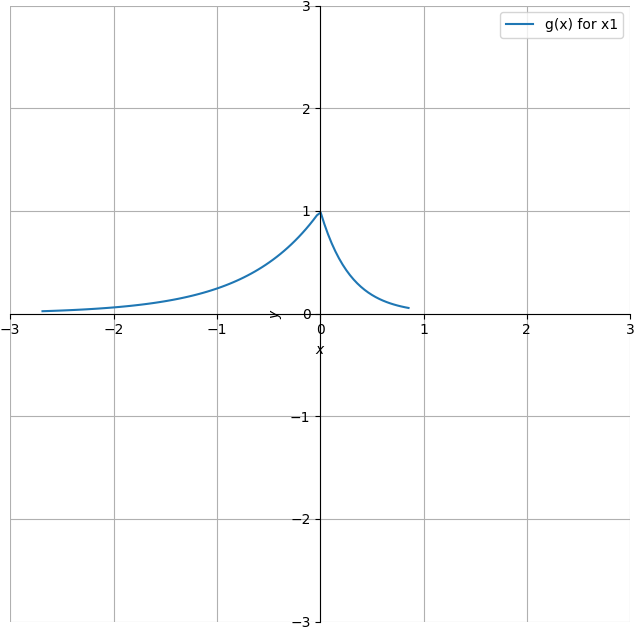
\includegraphics[width=0.7\columnwidth]{figs/trunc.png}
	\caption{}
	\label{fig:Truncation}
\end{figure}

\newpage
\appendices
\section{Derivations}
\subsection{Linear Forms}
\begin{enumerate}[label=\thesubsection.\arabic*.,ref=\thesubsection.\theenumi]
\item Let $\vec{Q}$ be the foot of the perpendicular from $\vec{P}$
	to the line
\begin{align}
			\label{eq:geo-norm-app}
    \vec{n}^{\top}  \vec{x} = c
\end{align}
Then
\begin{align}
PQ =  
	\frac{\abs{\vec{n}^{\top}\vec{P} - c}}{\norm{\vec{n}}}
			\label{eq:PQ-final}
\end{align}
	\item 
The affine transformation is given by 
\begin{align}
	\label{eq:conic_affine}
	\vec{x} = \vec{P}\vec{y}+\vec{c}
\end{align}
where $\vec{c}$ is the translation vector.
\end{enumerate}
\subsection{Eigenvalues and Eigenvectors}
\begin{enumerate}[label=\thesubsection.\arabic*.,ref=\thesubsection.\theenumi]
	\item The roots of the equation are known as the eigenvalues of $\vec{\Sigma}$.
\begin{align}
	\mydet{\lambda \vec{I}-\vec{\Sigma}} = 0
\end{align}
\item The values of $\vec{p}$ that satisfy
\begin{align}
	\vec{\Sigma}\vec{p}
	=\lambda\vec{p}
\end{align}
are known as the eigenvectors of $\Sigma$.
\item Define
    \begin{align}
      \label{eq:conic_parmas_eig_def-D}
      \vec{D} &= \myvec{\lambda_1 & 0\\ 0 & \lambda_2}, 
      \\
	    \vec{P} &= \myvec{\frac{\vec{p}_1}{\norm{\vec{p}_1}} & \frac{\vec{p}_2}{\norm{\vec{p}_2}}}
      \label{eq:eigevecP}
    \end{align}
    \item Note that
  \begin{align}
\vec{P}^{\top}=\vec{P}^{-1}.
  \label{eq:orth-mat}
  \end{align}
  $\vec{P}$ is defined to be an orthogonal matrix.
\item Note that
    \begin{align}
      \label{eq:conic_parmas_eig_def}
      \vec{P}^{\top}\vec{\Sigma}\vec{P} &= \vec{D},
    \end{align} 
		This is known as the spectral (eigenvalue) decomposition of a symmetric matrix 
	\item For a symmetric matrix, from \eqref{eq:conic_parmas_eig_def}, we have the eigendecomposition
\begin{align}
	\vec{V}&=\vec{P}\vec{D}
      \label{eq:conic_eig_def}
\vec{P}^{\top}
\end{align}
where 
%
\begin{align}
	\vec{P} &= \myvec{\vec{p}_1 & \vec{p}_2}, \quad 
\vec{P}^{\top}\vec{P} = 
	\vec{I}
\label{eq:eig_matrix}
\\
      \label{eq:D}
	  \vec{D} &= \myvec{\lambda_1 & 0 \\ 0 & \lambda_2}
\end{align}
\end{enumerate}
\subsection{Conic Section}
\begin{enumerate}[label=\thesubsection.\arabic*.,ref=\thesubsection.\theenumi]
\item
  Let $\vec{q}$ be a point such that the ratio of its distance from a fixed point $\vec{F}$ and the distance ($d$) from a fixed line 
	\begin{align}
L: \vec{n}^{\top}\vec{x}=c 
	\end{align}
		is constant, given by 
\label{conics/30/def}
\begin{align}
\frac{\norm{\vec{q}-\vec{F}}}{d} = e    
\end{align}
The locus of $\vec{q}$ is known as a conic section. The line $L$ is known as the directrix and the point $\vec{F}$ is the focus. $e$ is defined to be 
the eccentricity of the conic.  
\begin{enumerate}
    \item For $e = 1$, the conic is a parabola
    \item For $e < 1$, the conic is an ellipse
    \item For $e > 1$, the conic is a hyperbola
\end{enumerate}

\item
The equation of  a conic with directrix $\vec{n}^{\top}\vec{x} = c$, eccentricity $e$ and focus $\vec{F}$ is given by 
\begin{align}
    \label{eq:app-conic_quad_form}
	\text{g}\brak{\vec{x}} = \vec{x}^{\top}\vec{V}\vec{x}+2\vec{u}^{\top}\vec{x}+f=0
    \end{align}
where     
\begin{align}
  \label{eq:app-conic_quad_form_v}
\vec{V} &=\norm{\vec{n}}^2\vec{I}-e^2\vec{n}\vec{n}^{\top}, 
\\
\label{eq:app-conic_quad_form_u}
\vec{u} &= ce^2\vec{n}-\norm{\vec{n}}^2\vec{F}, 
\\
\label{eq:app-conic_quad_form_f}
f &= \norm{\vec{n}}^2\norm{\vec{F}}^2-c^2e^2
    \end{align}
    \solution
  Using Definition \ref{conics/30/def} and 
			\eqref{eq:PQ-final},
for any point $\vec{x}$ on the conic,
\begin{align}
	\norm{\vec{x}-\vec{F}}^2&=e^2 \frac{\brak{{\vec{n}^{\top}\vec{x} - c}}^2}{\norm{\vec{n}}^2}\label{conics/30/eq:1} \\
	\implies \norm{\vec{n}}^2\brak{\vec{x}-\vec{F}}^{\top}\brak{\vec{x}-\vec{F}}&=e^2\brak{\vec{n}^{\top}\vec{x} - c}^2
\\
\implies \norm{\vec{n}}^2\brak{\vec{x}^{\top}\vec{x}-2\vec{F}^{\top}\vec{x}+\norm{\vec{F}}^2}
	&=e^2\brak{c^2+\brak{\vec{n}^{\top}\vec{x} }^2-2c\vec{n}^{\top}\vec{x}} \\
	&=e^2\brak{c^2+\brak{\vec{x}^{\top}\vec{n}\vec{n}^{\top}\vec{x} }-2c\vec{n}^{\top}\vec{x}}
\end{align}
%
which can be expressed as \eqref{eq:app-conic_quad_form} after simplification.
\item
  The eccentricity, directrices and foci of \eqref{eq:app-conic_quad_form} are given by 
\begin{align}
  \label{eq:app-conic_quad_form_e} 
  e&= \sqrt{1-\frac{\lambda_1}{\lambda_2}}
\\
\label{eq:app-conic_quad_form_nc} 
	\begin{split}
  \vec{n}&= \sqrt{\lambda_2}\vec{p}_1,  
  \\
	c &= 
  \begin{cases}
    \frac{e\vec{u}^{\top}\vec{n} \pm \sqrt{e^2\brak{\vec{u}^{\top}\vec{n}}^2-\lambda_2\brak{e^2-1}\brak{\norm{\vec{u}}^2 - \lambda_2 f}}}{\lambda_2e\brak{e^2-1}} & e \ne 1
    \\
    \frac{\norm{\vec{u}}^2 - \lambda_2 f   }{2\vec{u}^{\top}\vec{n}} & e = 1
  \end{cases}
	\end{split}
  \\
  \label{eq:app-conic_quad_form_F} 
  \vec{F}  &= \frac{ce^2\vec{n}-\vec{u}}{\lambda_2}
\end{align}  
	\label{app:conic-parameters}
	\solution
	From \eqref{eq:app-conic_quad_form_v}, using the fact that $\vec{V}$ is symmetric with $\vec{V} = \vec{V}^{\top}$,
  \begin{align}
	  \vec{V}^{\top} \vec{V}&=\brak{\norm{\vec{n}}^2\vec{I}-e^2\vec{n}\vec{n}^{\top}}^{\top}
	  \brak{\norm{\vec{n}}^2\vec{I}-e^2\vec{n}\vec{n}^{\top}}
    \\
	  \implies \vec{V}^{2} &= \norm{\vec{n}}^4\vec{I}+e^4\vec{n}\vec{n}^{\top}\vec{n}\vec{n}^{\top}
	  -2e^2\norm{\vec{n}}^2\vec{n}\vec{n}^{\top}
    \\
	  &= \norm{\vec{n}}^4\vec{I} + e^4\norm{\vec{n}}^2\vec{n}\vec{n}^{\top}
	%  \\
	  - 2e^2\norm{\vec{n}}^2\vec{n}\vec{n}^{\top}
    \\
	  &= \norm{\vec{n}}^4\vec{I} + e^2\brak{e^2 - 2}\norm{\vec{n}}^2\vec{n}\vec{n}^{\top}
    \\
	  &= \norm{\vec{n}}^4\vec{I} + \brak{e^2 - 2}\norm{\vec{n}}^2\brak{\norm{\vec{n}}^2\vec{I}- \vec{V}}
    \end{align}
%    
which can be expressed as
\begin{align}
  \vec{V}^{2} + \brak{e^2 - 2}\norm{\vec{n}}^2\vec{V} - \brak{e^2 - 1}\norm{\vec{n}}^4\vec{I}=0
  \label{eq:app-conic_quad_form_e_cayley}
\end{align}
	Using the Cayley-Hamilton theorem,
	\eqref{eq:app-conic_quad_form_e_cayley} results in the characteristic equation, 
\begin{align}
  \lambda^{2} - \brak{2-e^2}\norm{\vec{n}}^2\lambda + \brak{1-e^2 }\norm{\vec{n}}^4=0
\end{align}
which can be expressed as
\begin{align}
\brak{\frac{\lambda}{\norm{\vec{n}}^2}}^2 - \brak{2-e^2 }\brak{\frac{\lambda}{\norm{\vec{n}}^2}} 
	+ \brak{1-e^2 } = 0
	\\
	\implies \frac{\lambda}{\norm{\vec{n}}^2} = 1-e^2, 1
  \\
	\text{or, }\lambda_2 = \norm{\vec{n}}^2, \lambda_1 = \brak{1-e^2}\lambda_2 
  \label{eq:app-conic_quad_form_lam_cayley}
\end{align}
From   \eqref{eq:app-conic_quad_form_lam_cayley}, the eccentricity of \eqref{eq:app-conic_quad_form} is given by 
\eqref{eq:app-conic_quad_form_e}.   
%
Multiplying both sides of    \eqref{eq:app-conic_quad_form_v} by $\vec{n}$,
\begin{align}
\vec{V} \vec{n}&=\norm{\vec{n}}^2\vec{n}-e^2\vec{n}\vec{n}^{\top}\vec{n} 
\\
&=\norm{\vec{n}}^2\brak{1-e^2}\vec{n} 
 \\
  &=\lambda_1 \vec{n} 
	\\
  \label{eq:eigevecn}
\end{align}  
from \eqref{eq:app-conic_quad_form_lam_cayley}.
Thus,  $\lambda_1$ is the corresponding eigenvalue for $\vec{n}$.  From       \eqref{eq:eigevecP} and \eqref{eq:eigevecn}, this implies that 
\begin{align}  
	\vec{p}_1 &= \frac{\vec{n}}{\norm{\vec{n}}} 
	\\
	\text{or, }
   \vec{n}&= \norm{\vec{n}}\vec{p}_1  = \sqrt{\lambda_2}\vec{p}_1 
\end{align}  
from   \eqref{eq:app-conic_quad_form_lam_cayley} .
From \eqref{eq:app-conic_quad_form_u} and \eqref{eq:app-conic_quad_form_lam_cayley},
\begin{align}
\vec{F}  &= \frac{ce^2\vec{n}-\vec{u}}{\lambda_2}
 \\
 \implies \norm{\vec{F}}^2  &= \frac{\brak{ce^2\vec{n}-\vec{u}}^{\top}\brak{ce^2\vec{n}-\vec{u}}}{\lambda_2^2}
 \\
 \implies \lambda_2^2\norm{\vec{F}}^2  &= c^2e^4\lambda_2-2ce^2\vec{u}^{\top}\vec{n}+\norm{\vec{u}}^2
 \label{eq:app-conic_quad_form_u_temp}
    \end{align}
    Also, \eqref{eq:app-conic_quad_form_f} can be expressed as
    \begin{align}
    \lambda_2\norm{\vec{F}}^2 &= f+c^2e^2
    \label{eq:app-conic_quad_form_f_temp}
\end{align}
From  \eqref{eq:app-conic_quad_form_u_temp} and     \eqref{eq:app-conic_quad_form_f_temp},
\begin{align}
c^2e^4\lambda_2-2ce^2\vec{u}^{\top}\vec{n}+\norm{\vec{u}}^2 = \lambda_2\brak{f+c^2e^2}
\end{align}
\begin{align}
\implies \lambda_2e^2\brak{e^2-1}c^2-2ce^2\vec{u}^{\top}\vec{n}
	+\norm{\vec{u}}^2 - \lambda_2 f = 0
\end{align}
yielding
  \eqref{eq:app-conic_quad_form_F}. 
\item
\eqref{eq:app-conic_quad_form} represents 
	\begin{enumerate}
		\item a parabola for $\mydet{\vec{V}} = 0 $,
		\item ellipse for $\mydet{\vec{V}} > 0 $ and 
		\item hyperbola for $\mydet{\vec{V}} < 0 $.
	\end{enumerate}
\solution
  From \eqref{eq:app-conic_quad_form_e},
\begin{align}
  \frac{\lambda_1}{\lambda_2} = 1 - e^2
\end{align}
Also, 
\begin{align}
	\mydet{\vec{V}} =   \lambda_1\lambda_2 
\end{align}
	yielding \tabref{table:det}.
\begin{table}[H]
\centering
\resizebox{\columnwidth}{!}{%
\input{tables/det.tex}
	}
	\caption{}
\label{table:det}
\end{table}
			\item Using the affine transformation in
					\label{app:std-prm-P}
	\eqref{eq:conic_affine},
	the conic in     \eqref{eq:app-conic_quad_form} can be expressed in standard form 
	%(centre/vertex at the origin, major axis - $x$ axis)
	as
  \begin{align}
    %\begin{aligned}
    \label{eq:app-conic_simp_temp_nonparab}
	    \vec{y}^{\top}\brak{\frac{\vec{D}}{f_0}}\vec{y} &= 1   &  \abs{\vec{V}} &\ne 0
    \\
	    \vec{y}^{\top}\vec{D}\vec{y} &=  -\eta\vec{e}_1^{\top}\vec{y}   & \abs{\vec{V}} &= 0
    \label{eq:app-conic_simp_temp_parab}
    %\end{aligned}
    \end{align}
    where
  \begin{align}
      %\begin{split}
      \label{eq:app-f0}
	  f_0 &=\vec{u}^{\top}\vec{V}^{-1}\vec{u} -f \ne 0
	  \\
      \label{eq:app-eta}
       \eta &=2\vec{u}^{\top}\vec{p}_1
       \\
       \vec{e}_1 &=\myvec{1 \\ 0}
      \end{align}
      \solution
  \label{app:parab}
	Using 
\eqref{eq:conic_affine},
\eqref{eq:app-conic_quad_form} can be expressed as
\begin{align}
\brak{\vec{P}\vec{y}+\vec{c}}^{\top}\vec{V}\brak{\vec{P}\vec{y}+\vec{c}}+2\vec{u}^{\top}\brak{\vec{P}\vec{y}+\vec{c}}+ f
	= 0, 
\end{align}
yielding 
\begin{align}
\vec{y}^{\top}\vec{P}^{\top}\vec{V}\vec{P}\vec{y}+2\brak{\vec{V}\vec{c}+\vec{u}}^{\top}\vec{P}\vec{y}
+  \vec{c}^{\top}\vec{V}\vec{c} + 2\vec{u}^{\top}\vec{c} + f= 0
\label{eq:conic_simp_one}
\end{align}
%
From \eqref{eq:conic_simp_one} and \eqref{eq:conic_parmas_eig_def},
\begin{align}
\vec{y}^{\top}\vec{D}\vec{y}+2\brak{\vec{V}\vec{c}+\vec{u}}^{\top}\vec{P}\vec{y}
+  \vec{c}^{\top}\brak{\vec{V}\vec{c} + \vec{u}}+ \vec{u}^{\top}\vec{c} + f= 0
\label{eq:conic_simp}
\end{align}
When $\vec{V}^{-1}$ exists, choosing
\begin{align}
%\begin{split}
\vec{V}\vec{c}+\vec{u} &= \vec{0}, \quad \text{or}, \vec{c} = -\vec{V}^{-1}\vec{u},
\label{eq:conic_parmas_c_def}
\end{align}
%
%%From \eqref{eq:conic_parmas_k_def} and 
%%
and substituting \eqref{eq:conic_parmas_c_def}
in \eqref{eq:conic_simp}
yields \eqref{eq:app-conic_simp_temp_nonparab}. 
  %See Appendix \ref{app:parab}.
When $\abs{\vec{V}} = 0, \lambda_1 = 0$ and 
\begin{align}
\vec{V}\vec{p}_1 = 0, 
\vec{V}\vec{p}_2 = \lambda_2\vec{p}_2.
\label{eq:conic_parab_eig_prop} 
\end{align}
Substituting \eqref{eq:eig_matrix}
in \eqref{eq:conic_simp},
\begin{align*}
	\vec{y}^{\top}\vec{D}\vec{y}+2\brak{\vec{c}^{\top}\vec{V}+\vec{u}^{\top}}\myvec{\vec{p}_1 & \vec{p}_2}\vec{y}
%	\\
	+  \vec{c}^{\top}\brak{\vec{V}\vec{c} + \vec{u}}+ \vec{u}^{\top}\vec{c} + f= 0
\\
\implies \vec{y}^{\top}\vec{D}\vec{y}
+2\myvec{\brak{\vec{c}^{\top}\vec{V}+\vec{u}^{\top}}\vec{p}_1  \brak{\vec{c}^{\top}\vec{V}+\vec{u}^{\top}}\vec{p}_2}\vec{y}
%\\
	+  \vec{c}^{\top}\brak{\vec{V}\vec{c} + \vec{u}}+ \vec{u}^{\top}\vec{c} + f= 0
\\
\implies \vec{y}^{\top}\vec{D}\vec{y}
+2\myvec{\vec{u}^{\top}\vec{p}_1 & \brak{\lambda_2\vec{c}^{\top}+\vec{u}^{\top}}\vec{p}_2}\vec{y}
%\\
	+  \vec{c}^{\top}\brak{\vec{V}\vec{c} + \vec{u}}+ \vec{u}^{\top}\vec{c} + f= 0
\end{align*}
upon substituting from 
 \eqref{eq:conic_parab_eig_prop}, yielding
\begin{multline}
\lambda_2y_2^2+2\brak{\vec{u}^{\top}\vec{p}_1}y_1+  2y_2\brak{\lambda_2\vec{c}+\vec{u}}^{\top}\vec{p}_2
%\\
	+  \vec{c}^{\top}\brak{\vec{V}\vec{c} + \vec{u}}+ \vec{u}^{\top}\vec{c} + f= 0
\label{eq:conic_parab_foc_len_temp} 
\end{multline}
%which is the equation of a parabola. 
Thus, \eqref{eq:conic_parab_foc_len_temp} 
can be expressed as \eqref{eq:app-conic_simp_temp_parab} by choosing
\begin{align}
%\label{eq:app-eta}
\eta = 2\vec{u}^{\top}\vec{p}_1
\end{align}
%Choosing 
%\begin{align}
%\vec{u} + \lambda_2\vec{c} = 0,
%\vec{c}^{\top}\brak{\vec{V}\vec{c} + \vec{u}}+ \vec{u}^{\top}\vec{c} + f = 0,
%\end{align}
% the above equation becomes
%\begin{align}
%y_2^2= -\frac{2\vec{u}^{\top}\vec{p}_1}{ \lambda_2} \brak{y_1
%+  \frac{\vec{u}^{\top}\vec{V}\vec{u} - 2\lambda_2\vec{u}^{\top}\vec{u} + f\lambda_2^2}{2\vec{u}^{\top}\vec{p}_1\lambda_2^2}}
%\\
%or \eta = 2\vec{u}^{\top}\vec{p}_1
%%\label{eq:conic_simp_parab_new}
%\end{align}
and $\vec{c}$ in \eqref{eq:conic_simp} such that
\begin{align}
\label{eq:conic_parab_one}
2\vec{P}^{\top}\brak{\vec{V}\vec{c}+\vec{u}} &= \eta\myvec{1\\0}
\\
\vec{c}^{\top}\brak{\vec{V}\vec{c} + \vec{u}}+ \vec{u}^{\top}\vec{c} + f&= 0
\label{eq:conic_parab_two}
\end{align}
%we obtain  \eqref{eq:app-conic_simp_temp_parab}.
	\item
		The center/vertex of a conic section are given by
  \begin{align}
    \label{eq:app-conic_nonparab_c}
	    \vec{c} &= - \vec{V}^{-1}\vec{u}  & \mydet{\vec{V}} \ne 0
    \\
	    \myvec{ \vec{u}^{\top}+\frac{\eta}{2}\vec{p}_1^{\top} \\ \vec{V}}\vec{c} &= \myvec{-f \\ \frac{\eta}{2}\vec{p}_1-\vec{u}}  
& \mydet{\vec{V}} = 0
    \label{eq:conic_parab_c}
    \end{align}	
\solution	
$\because
\vec{P}^{\top}\vec{P} = \vec{I}$,
multiplying \eqref{eq:conic_parab_one} by $\vec{P}$ yields
\begin{align}
\label{eq:conic_parab_one_eig}
	\brak{\vec{V}\vec{c}+\vec{u}} &= \frac{\eta}{2}\vec{p}_1,
\end{align}
which, upon substituting in \eqref{eq:conic_parab_two}
results in 
\begin{align}
\frac{\eta}{2}\vec{c}^{\top}\vec{p}_1 + \vec{u}^{\top}\vec{c} + f&= 0
\label{eq:conic_parab_two_eig}
\end{align}
\eqref{eq:conic_parab_one_eig} and \eqref{eq:conic_parab_two_eig} can be clubbed together to obtain \eqref{eq:conic_parab_c}.
\item
			In 
			\eqref{eq:conic_affine}, substituting $\vec{y} = \vec{0}$, the center/vertex for the quadratic form is obtained as
    \begin{align}
	    \vec{x} = \vec{c}, 
    \end{align}
			where $\vec{c}$ is derived as 
    \eqref{eq:app-conic_nonparab_c}
    and 
    \eqref{eq:conic_parab_c}
in Appendix  \ref{app:parab}.
 \item
	 \label{prop:chord}
  The points of intersection of the line 
\begin{align}
L: \quad \vec{x} = \vec{h} + \kappa \vec{m} \quad \kappa \in \mathbb{R}
\label{eq:app-conic_tangent}
\end{align}
with the conic section in \eqref{eq:app-conic_quad_form} are given by
\begin{align}
\vec{x}_i = \vec{h} + \kappa_i \vec{m}
	\label{eq:app-chord-pts}
\end{align}
%
where
\begin{multline}
\kappa_i = \frac{1}
{
\vec{m}^{\top}\vec{V}\vec{m}
}
\lbrak{-\vec{m}^{\top}\brak{\vec{V}\vec{h}+\vec{u}}}
%\\
\pm
%{\small
\rbrak{\sqrt{
\sbrak{
\vec{m}^{\top}\brak{\vec{V}\vec{h}+\vec{u}}
}^2
	-\text{g}
\brak
{\vec{h}
%\vec{h}^{\top}\vec{V}\vec{h} + 2\vec{u}^{\top}\vec{h} +f
}
\brak{\vec{m}^{\top}\vec{V}\vec{m}}
}
}
%}
\label{eq:app-tangent_roots}
\end{multline}
\solution
  Substituting \eqref{eq:app-conic_tangent}
in \eqref{eq:app-conic_quad_form}, 
\begin{align}
\brak{\vec{h} + \kappa \vec{m}}^{\top}\vec{V}\brak{\vec{h} + \kappa \vec{m}}  + 2 \vec{u}^{\top}\brak{\vec{h} + \kappa \vec{m}}+f &= 0
\\
\implies \kappa^2\vec{m}^{\top}\vec{V}\vec{m} + 2 \kappa\vec{m}^{\top}\brak{\vec{V}\vec{h}+\vec{u}} 
+ \vec{h}^{\top}\vec{V}\vec{h} + 2\vec{u}^{\top}\vec{h} +f &= 0
	\\
	\text{or, }
\kappa^2\vec{m}^{\top}\vec{V}\vec{m} + 2 \kappa\vec{m}^{\top}\brak{\vec{V}\vec{h}+\vec{u}} 
	+ \text{g}\brak{\vec{h}} &=0
	%^{\top}\vec{V}\vec{h} + 2\vec{u}^{\top}\vec{h} +f &= 0
\label{eq:conic_intercept}
\end{align}
for g defined in \eqref{eq:app-conic_quad_form}.
Solving the above quadratic in \eqref{eq:conic_intercept}
yields \eqref{eq:app-tangent_roots}.
		\end{enumerate}


\end{document}
